% Author: Izaak Neutelings (February 2019)
% Inspiration: https://tex.stackexchange.com/questions/285578/how-to-draw-parallelepiped-and-cube-with-latex/288101#288101
\documentclass[border=3pt,tikz]{standalone}
\usetikzlibrary{quotes,arrows,arrows.meta}
\tikzset{>=latex} % for LaTeX arrow head

\colorlet{myblue}{blue!20}
\colorlet{mydarkblue}{blue!50!black}
\colorlet{myred}{black!50!red}

% CUBE
\tikzset{
  cube/.pic={
    \tikzset{every edge quotes/.append style={midway,auto},/cube/.cd,#1}
    \def\csize{2*\cubesize}
    \draw [every edge/.append style={pic actions,densely dashed,opacity=.5},pic actions]
    (0,0,0) coordinate (o)
            edge coordinate [pos=1] (g) ++(0,0,-\csize)
        --++(0,\csize,0) coordinate (a)
        --++(\csize,0,0) coordinate (b)
        --++(0,-\csize,0) coordinate (c) -- cycle
    (a) --++(0,0,-\csize) coordinate (d) edge (g)
        --++(\csize,0,0) coordinate (e) -- (b) -- cycle
    (c) -- (b) -- (e)
        --++(0,-\csize,0) coordinate (f) edge (g) -- cycle;
    \path [every edge/.append style={pic actions, |-|}];
  },
  z={(-0.334,-0.334)},
  /cube/.search also={/tikz},
  /cube/.cd,
  size/.store in=\cubesize, size=1,
}

% GAS MOLECULE with vector
\tikzset{
  gasparticle/.pic={
    \tikzset{/gasparticle/.cd,#1}
    \draw[->,green!60!black] (0,0) -- (\vec);
    \node[circle,fill,inner sep=.8,fill=black!80!blue] at (0,0,0) {};
  }
  /gasparticle/.search also={/tikz},
  /gasparticle/.cd,
  vec/.store in=\vec, vec={90:0.5},
}



\begin{document}

% GAS in a box
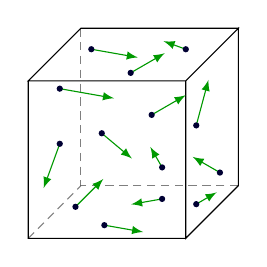
\begin{tikzpicture}
  \pic at (0,0,0) {cube={size=1}};
  \pic at (0.6,1.0,-1.0) {gasparticle={vec={-40:0.5}}};
  \pic at (0.2,1.0,-0.6) {gasparticle={vec={-110:0.6}}};
  \pic at (0.2,1.7,-0.6) {gasparticle={vec={-10:0.7}}};
  \pic at (0.5,0.3,-0.3) {gasparticle={vec={45:0.5}}};
  \pic at (0.9,0.1,-0.2) {gasparticle={vec={-10:0.5}}};
  \pic at (1.6,0.4,-0.3) {gasparticle={vec={-170:0.4}}};
  \pic at (1.5,1.9,-1.5) {gasparticle={vec={160:0.3}}};
  \pic at (0.2,1.8,-1.8) {gasparticle={vec={-10:0.6}}};
  \pic at (1.4,0.6,-0.9) {gasparticle={vec={120:0.3}}};
  \pic at (0.8,1.6,-1.5) {gasparticle={vec={30:0.5}}};
  \pic at (1.8,1.1,-1.0) {gasparticle={vec={75:0.6}}};
  \pic at (1.8,0.2,-1.9) {gasparticle={vec={150:0.4}}};
  \pic at (1.9,0.2,-0.7) {gasparticle={vec={30:0.3}}};
  \pic at (1.2,1.2,-1.1) {gasparticle={vec={30:0.5}}};
\end{tikzpicture}

% GAS - macroscopic
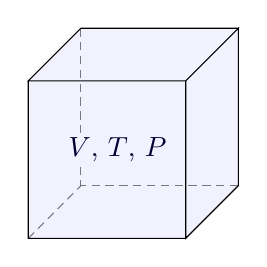
\begin{tikzpicture}
  \pic[fill=blue!5] at (0,0,0) {cube={size=1}};
  \node[below,black!80!blue,fill=blue!5,inner sep=0pt] at (0.8,0.95,-1) {$V$, $T$, $P$};
  %\draw[-,black!80!blue] (2,1,-1) -- (2.5,1,-1) node[right,black!80!blue] (2,1,-1) {$A$};
\end{tikzpicture}

% DIATOMIC
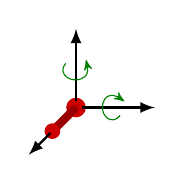
\begin{tikzpicture}[z={(-0.6,-0.6)}]
  \node[circle,fill,inner sep=2.5,fill=red!80!black] at (0,0,0) {};
  \node[circle,fill,inner sep=1.07,fill=red!60!black] at (0,0,0.04) {};
  \draw[red!60!black,line width=3] (0,0,0.04) -- (0,0,0.5);
  \node[circle,fill,inner sep=2,fill=red!80!black] at (0,0,0.5) {};
  \draw[->,thick] (0.08,0,0) -- (1,0,0);
  \draw[->,thick] (0,0.08,0) -- (0,1,0);
  \draw[->,thick] (0,0,0.54) -- (0,0,1);
  \draw[->,>=stealth',shorten >=-3pt,green!50!black,yscale=0.8]
    (-0.13,0.7,0) arc[radius=0.16,start angle=-220,end angle=10];
  \draw[->,>=stealth',shorten >=-3pt,green!50!black,xscale=0.8]
    (0.7,-0.1,0) arc[radius=0.16,start angle=-40,end angle=-300];
\end{tikzpicture}

% HOT BALLOON
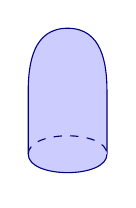
\begin{tikzpicture}[yscale=0.8]
  \draw[mydarkblue,fill=myblue]
    (-.5,0) -- (-.5,1) to[out=90,in=180] (0,2) to[out=0,in=90] (.5,1) -- (.5,0);
  \draw[dashed,mydarkblue,fill=myblue]
    (-.5,0) to[out=90,in=90] (.5,0);
  \draw[mydarkblue,fill=myblue]
    (-.5,0) to[out=-90,in=-90] (.5,0);
\end{tikzpicture}

% GAS in a box - partioned
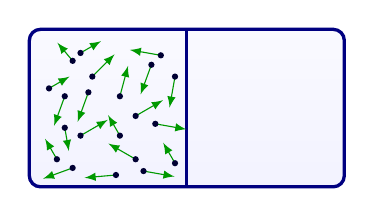
\begin{tikzpicture}
  \draw[mydarkblue,very thick,rounded corners=4,
        top color=blue!2,bottom color=blue!5,shading angle=0]
    (0,0) rectangle (4,2);
  \draw[mydarkblue,very thick] (2,0) --++ (0,2);
  %\draw[blue!50,dashed] (1,0) --++ (0,2);
  %\draw[blue!50,dashed] (3,0) --++ (0,2);
  %\draw[blue!50,dashed] (0,1) --++ (4,0);
  %\draw[blue!50,dashed] (0,0.5) --++ (4,0);
  %\draw[blue!50,dashed] (0,1.5) --++ (4,0);
  \pic at (0.25,1.25) {gasparticle={vec={  30:0.3}}};
  \pic at (0.35,0.35) {gasparticle={vec={ 120:0.3}}};
  \pic at (0.45,1.15) {gasparticle={vec={-110:0.4}}};
  \pic at (0.45,0.75) {gasparticle={vec={ -80:0.3}}};
  \pic at (0.55,0.24) {gasparticle={vec={-160:0.4}}};
  \pic at (0.55,1.60) {gasparticle={vec={ 130:0.3}}};
  \pic at (0.65,0.65) {gasparticle={vec={  30:0.4}}};
  \pic at (0.65,1.70) {gasparticle={vec={  30:0.3}}};
  \pic at (0.80,1.40) {gasparticle={vec={  45:0.4}}};
  \pic at (0.75,1.20) {gasparticle={vec={-110:0.4}}};
  \pic at (1.10,0.15) {gasparticle={vec={-175:0.4}}};
  \pic at (1.15,0.65) {gasparticle={vec={ 120:0.3}}};
  \pic at (1.15,1.15) {gasparticle={vec={  75:0.4}}};
  \pic at (1.35,0.90) {gasparticle={vec={  30:0.4}}};
  \pic at (1.35,0.35) {gasparticle={vec={ 150:0.4}}};
  \pic at (1.45,0.20) {gasparticle={vec={ -10:0.4}}};
  \pic at (1.55,1.55) {gasparticle={vec={-110:0.4}}};
  \pic at (1.60,0.80) {gasparticle={vec={ -10:0.4}}};
  \pic at (1.67,1.67) {gasparticle={vec={ 170:0.4}}};
  \pic at (1.85,0.30) {gasparticle={vec={ 120:0.3}}};
  \pic at (1.85,1.40) {gasparticle={vec={-100:0.4}}};
\end{tikzpicture}

% GAS in a box - unpartioned
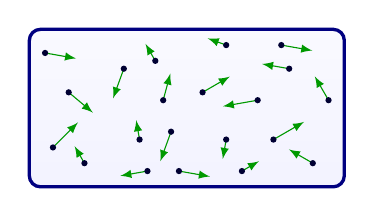
\begin{tikzpicture}
  \draw[mydarkblue,very thick,rounded corners=4,
        top color=blue!2,bottom color=blue!5,shading angle=0]
    (0,0) rectangle (4,2);
  \pic at (0.2,1.7) {gasparticle={vec={ -10:0.40}}};
  \pic at (0.3,0.5) {gasparticle={vec={  45:0.45}}};
  \pic at (0.5,1.2) {gasparticle={vec={ -40:0.40}}};
  \pic at (0.7,0.3) {gasparticle={vec={ 120:0.25}}};
  \pic at (1.2,1.5) {gasparticle={vec={-110:0.40}}};
  \pic at (1.4,0.6) {gasparticle={vec={ 100:0.25}}};
  \pic at (1.5,0.2) {gasparticle={vec={-170:0.35}}};
  \pic at (1.6,1.6) {gasparticle={vec={ 120:0.25}}};
  \pic at (1.7,1.1) {gasparticle={vec={  75:0.35}}};
  \pic at (1.8,0.7) {gasparticle={vec={-110:0.40}}};
  \pic at (1.9,0.2) {gasparticle={vec={ -10:0.40}}};
  \pic at (2.2,1.2) {gasparticle={vec={  30:0.40}}};
  \pic at (2.5,0.6) {gasparticle={vec={-100:0.25}}};
  \pic at (2.9,1.1) {gasparticle={vec={-170:0.45}}};
  \pic at (2.5,1.8) {gasparticle={vec={ 160:0.25}}};
  \pic at (2.7,0.2) {gasparticle={vec={  30:0.25}}};
  \pic at (3.1,0.6) {gasparticle={vec={  30:0.45}}};
  \pic at (3.2,1.8) {gasparticle={vec={ -10:0.40}}};
  \pic at (3.3,1.5) {gasparticle={vec={ 170:0.35}}};
  \pic at (3.6,0.3) {gasparticle={vec={ 150:0.35}}};
  \pic at (3.8,1.1) {gasparticle={vec={ 120:0.35}}};
\end{tikzpicture}

\end{document}